
%!TEX root = main.tex

%Main text
As mentioned above, we thought it would be helpful for you to get a basic overview of how our genetic system differs from yours. The important distinction to remember is that our species have a triploid genome that is made from combining three haploid gametes from our three parents (each of a distinct self-avoiding mating type), as opposed to your diploid genome that is made from combining two haploid gametes from your two parents.

\subsection*{Recombination}

In our species, each of our mating types makes a haploid gamete. The genetic material in this gamete is a third of the genetic material of its producer. Importantly, there is a recombination event that occurs before production of the gametes to ensure that there is genetic variation in the gamete pool. Homologous chromosomes are first aligned and bundled at their centers into a prism. Then several double strand breaks are made along each of the homologous chromosomes. Each broken strand is stabilized by the alignment of the other two chromosomes. The biological details of crossing over between two chromatids are similar to that of those observed on Earth. One or more exonucleases then digest nucleotides at the 5' end of each of the double strand breaks which allows for invasion of an opposite chromatid (Fig. \ref{fig:cross3}). The invading chromatid is determined by proximity to the broken chromatid in the prism. This invasion causes a displacement of the complimentary strand and a tetrahedral structure moves along the four-stranded structure. This tetrahedral structure proceeds by moving along the four strands and is then resolved by structure-selective nucleases. Each of the double strands breaks is resolved using the process detailed above. The chromosomal prism is then dissolved.       



%mention no recombination between sex genes
%end with recombined pre-gametes

\subsection*{Gamete formation and mating type determination}
As discussed previously, our species is composed of three self-avoiding mating types. These mating types are distinguished by three sex-determining genotypes: `XXY', `XYY' and `XYZ'. To illustrate gamete formation in our species, we will first describe the simplest case, which is that of gamete formation in our `female' species (genotype `XYZ'). 

Once the recombination event occurs, a cellular event analogous to what you call meiosis occurs to form haploid gametes, see Figure \ref{fig:meiosis_human}. In the case of our species however, there is an asymmetrical meiosis phase that we will call `Meiosis 0', see Figure \ref{fig:meiosis_us}, where the cells split in such a way that it forms a diploid daughter cell and a haploid daughter cell. The second step of our `Meiosis'-like event occurs only on the diploid cell and is analogous to your `Meiosis 1' step to form two haploid cells. All haploid cells then undergo a process analogous to `Meiosis 2' to form all the gametes.


\begin{figure}
    \centering
    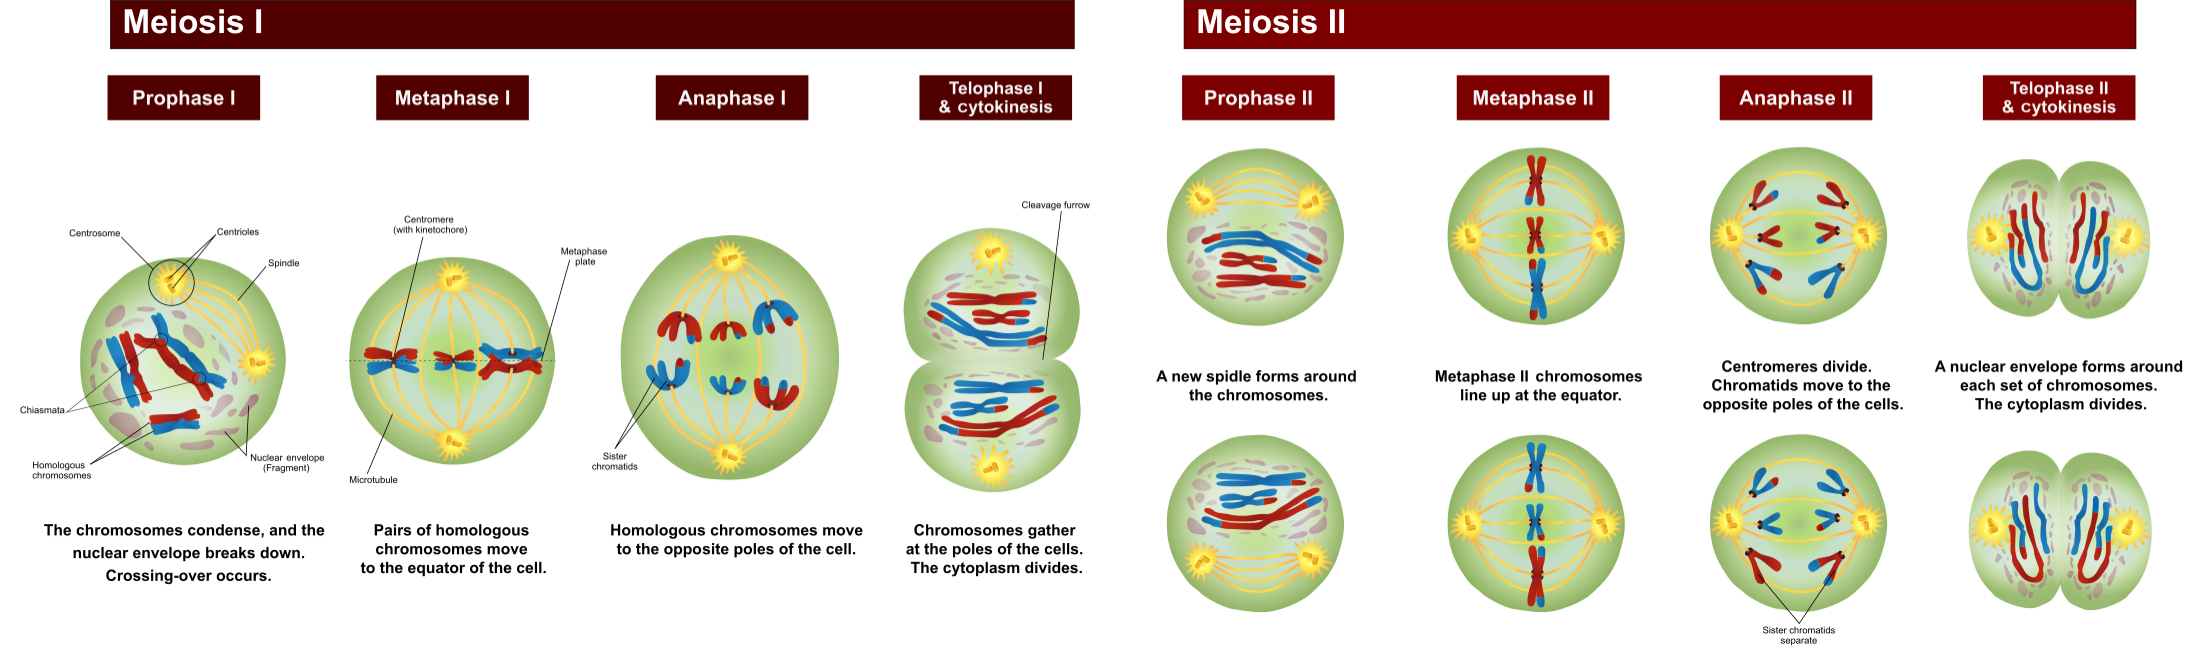
\includegraphics[width = 0.9\textwidth]{AshleyFig/meiosis3.png}
    \caption{Diagram of the phases of meiosis in humans and similar Earth-based life. Adapted from: Ali Zifan, CCA-SA 4.0}
    \label{fig:meiosis_human}
\end{figure}

\begin{figure}
    \centering
    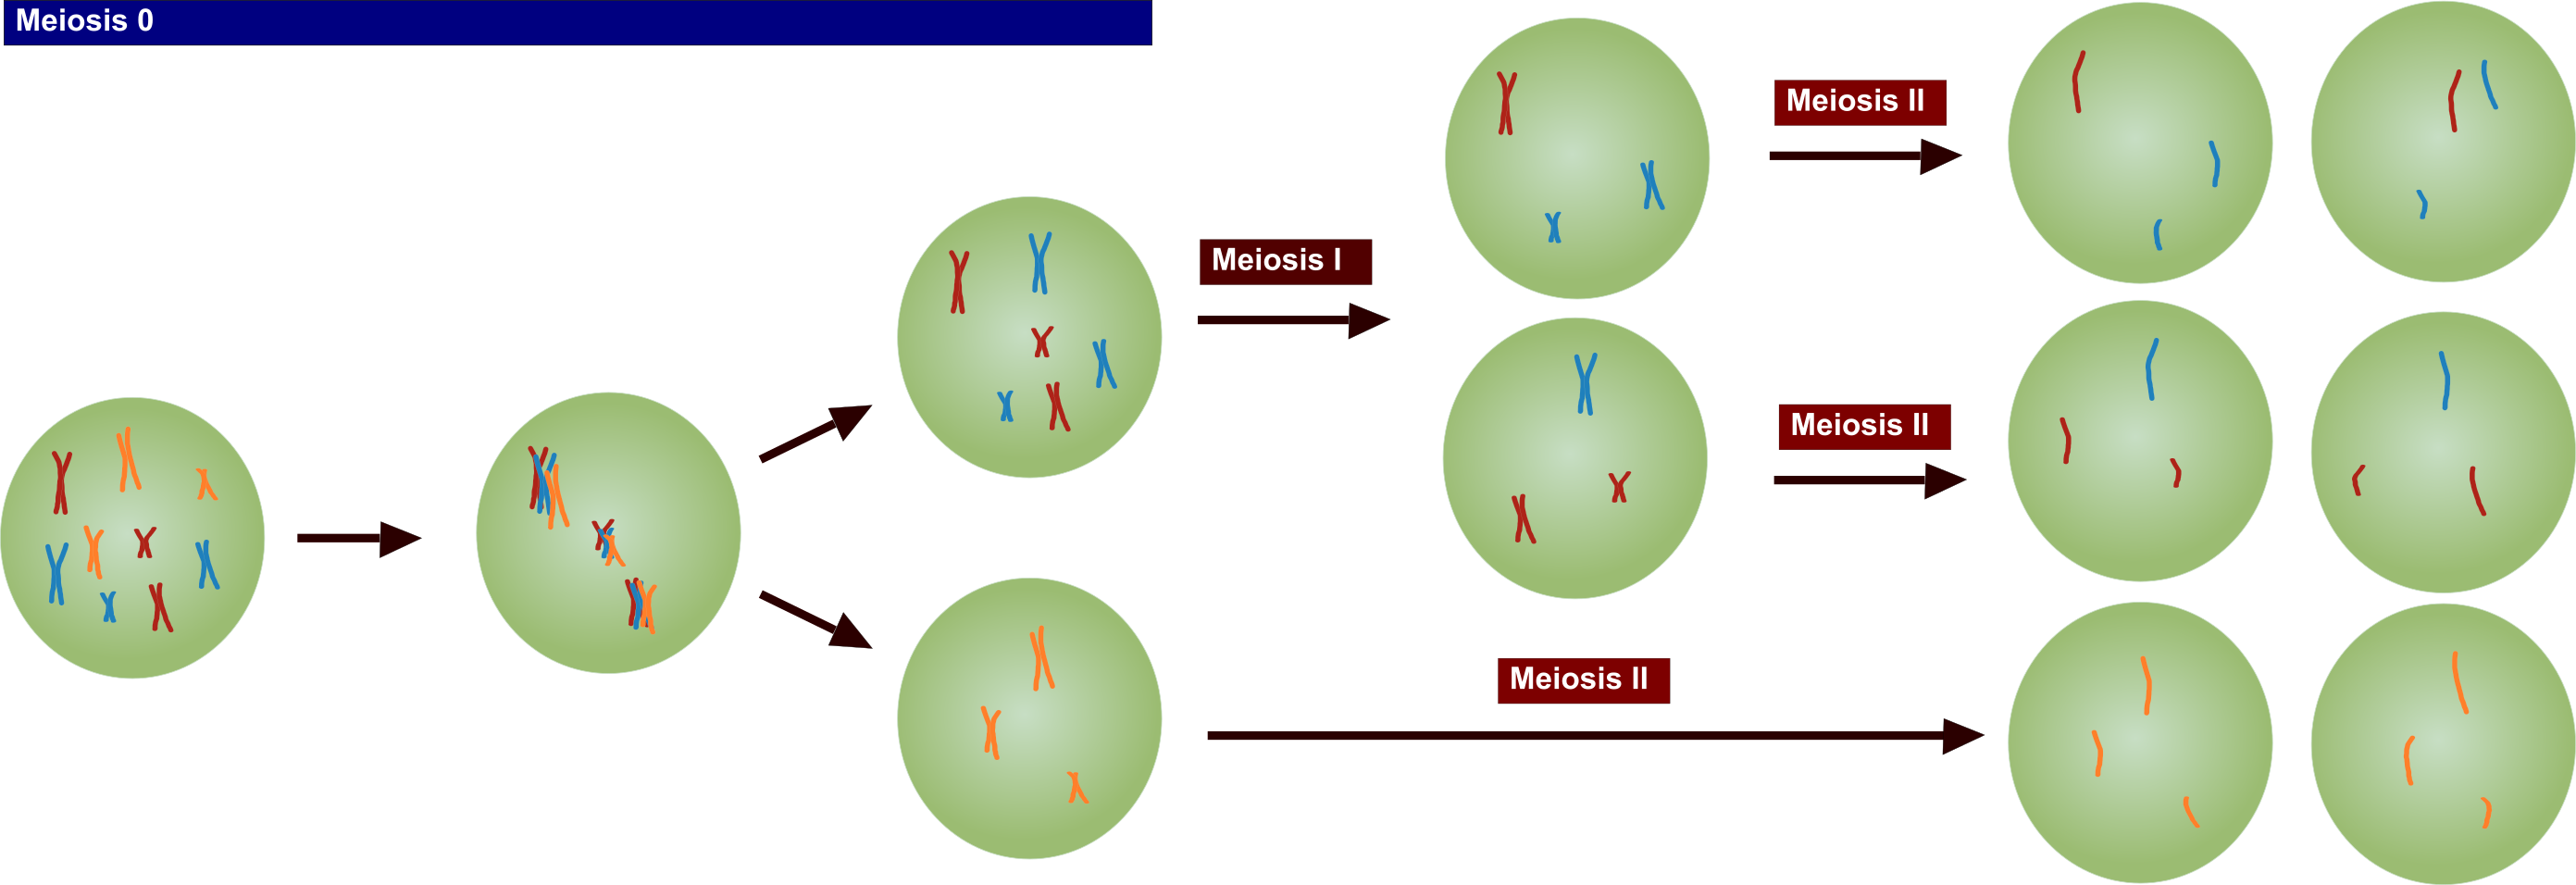
\includegraphics[width = 0.9\textwidth]{AshleyFig/meiosis0.png}
    \caption{Diagram of the phases of meiosis in our species. Intra-chromosomal recombination was not depicted here for clarity.}
    \label{fig:meiosis_us}
\end{figure}


This asymmetrical division, `Meiosis 0', crucially, is non-random in the two `male' mating types. The two `male' mating types (genotypes XXY and XYY) each have a pair of homologous sex-determining chromosomes (XX and YY respectively). In this case, unlike the fully heterologous XYZ female, the homologous pairs of chromosomes interact more strongly, causing them to always stay on the same side of the asymmetrical `Meiosis 0' step. This leads to the third sex-determining chromosome (Y and X respectively) to be separate and subsequently eliminated from the gamete formation process. In summary, genotype XXY only forms gametes with an X sex-determining chromosome while XYY only forms gametes with an Y sex-determining chromosome. In the heterologous XYZ female (with respect to sex-determining chromosomes), there is no elimination of cells that lead to gametes and as such, there is an even distribution of gametes with X, Y and Z sex-determining chromosomes in the gametes. Fertilization occurs when three gametes, each originating from a different mating type, meet and interact. The offspring's genetic material is thus a third of each of its parents. In conclusion, as illustrated in Table \ref{tab:punnet_us2}, the female's gamete determines the mating-type of the offspring, and all three mating-types are distributed evenly at birth.


\begin{table}
\centering
\begin{tikzpicture}[every node/.style={anchor=north east,fill=white,minimum width=.9cm,minimum height=.9mm}]
\matrix (mA) [draw,matrix of math nodes]
{
Xa & Xb & Xb & Yb \\
\hline
Yc & XXY & XXY &  \\
Yc & XXY & XXY &  \\
Xc &  &  &  \\
};

\matrix (mB) [draw,matrix of math nodes] at ($(mA.south west)+(.5,0.7)$)
{
Ya & Xb & Xb & Yb \\
\hline
Yc & YXY & YXY &  \\
Yc & YXY & YXY &  \\
Xc &  &  &  \\
};
x
\matrix (mC) [draw,matrix of math nodes] at ($(mB.south west)+(.5,0.7)$)
{
Za & Xb & Xb & Yb\\
\hline
Yc & ZXY & ZXY &  \\
Yc & ZXY & ZXY &  \\
Xc &  &  &  \\
};
\draw[dashed](mA.north east)--(mC.north east);
\draw[dashed](mA.north west)-- node[sloped,above] {} (mC.north west);
\draw[dashed](mA.south east)--(mC.south east);
\end{tikzpicture}
\caption{Partial Punnet cube of mating type assignment in our species. Letters a, b and c are used to help follow the three-mating types.} 
\label{tab:punnet_us2}
\end{table}




